%%%%%%%%%%%%%%%%%%%%%%%%%%%%%%%%%%%%%%%%%
% Journal Article
% LaTeX Template
% Version 1.3 (9/9/13)
%
% This template has been downloaded from:
% http://www.LaTeXTemplates.com
%
% Original author:
% Frits Wenneker (http://www.howtotex.com)
%
% License:
% CC BY-NC-SA 3.0 (http://creativecommons.org/licenses/by-nc-sa/3.0/)
%
%%%%%%%%%%%%%%%%%%%%%%%%%%%%%%%%%%%%%%%%%

%----------------------------------------------------------------------------------------
%	PACKAGES AND OTHER DOCUMENT CONFIGURATIONS
%----------------------------------------------------------------------------------------

\documentclass[twoside]{article}

%\usepackage[sc]{mathpazo} % Use the Palatino font
%\usepackage[T1]{fontenc} % Use 8-bit encoding that has 256 glyphs
%\linespread{1.05} % Line spacing - Palatino needs more space between lines
%\usepackage{microtype} % Slightly tweak font spacing for aesthetics

\usepackage[hmarginratio=1:1,top=32mm,columnsep=20pt]{geometry} % Document margins
\usepackage{multicol} % Used for the two-column layout of the document
\usepackage{appendix} % Use to add an appendix page to the document
\usepackage[hang, small,labelfont=bf,up,textfont=it,up]{caption} % Custom captions under/above floats in tables or figures
\usepackage{booktabs} % Horizontal rules in tables
\usepackage{float} % Required for tables and figures in the multi-column environment - they need to be placed in specific locations with the [H] (e.g. \begin{table}[H])
\usepackage{hyperref} % For hyperlinks in the PDF
\usepackage{amsmath} % Extra mathematical symbols and definitions
\usepackage{graphicx} % Include graphics
\geometry{letterpaper} % Scale for printing on 8.5"x11" paper

\usepackage{lettrine} % The lettrine is the first enlarged letter at the beginning of the text
\usepackage{paralist} % Used for the compactitem environment which makes bullet points with less space between them

\usepackage{abstract} % Allows abstract customization
\renewcommand{\abstractnamefont}{\normalfont\bfseries} % Set the "Abstract" text to bold
\renewcommand{\abstracttextfont}{\normalfont\small\itshape} % Set the abstract itself to small italic text

\usepackage{titlesec} % Allows customization of titles
\renewcommand\thesection{\Roman{section}} % Roman numerals for the sections
\renewcommand\thesubsection{\Roman{subsection}} % Roman numerals for subsections
\titleformat{\section}[block]{\large\scshape\centering}{\thesection.}{1em}{} % Change the look of the section titles
\titleformat{\subsection}[block]{\large}{\thesubsection.}{1em}{} % Change the look of the section titles

\usepackage{fancyhdr} % Headers and footers
\pagestyle{fancy} % All pages have headers and footers
\fancyhead{} % Blank out the default header
\fancyfoot{} % Blank out the default footer
\fancyhead[C]{Polytropes $\bullet$ April 21, 2014 } % Custom header text
\fancyfoot[RO,LE]{\thepage} % Custom footer text

\providecommand{\e}[1]{\ensuremath{\times 10^{#1}}}

%----------------------------------------------------------------------------------------
%	TITLE SECTION
%----------------------------------------------------------------------------------------

\title{\vspace{-15mm}\fontsize{24pt}{10pt}\selectfont\textbf{Polytropes and
Models of White Dwarf Stars}} % Article title

\author{
\large
\textsc{Erin Conn, Matthew Hurley}\\[2mm] % Your name
\normalsize University of North Carolina at Chapel Hill \\ % Your institution
\vspace{-5mm}
}
\date{}

%----------------------------------------------------------------------------------------

\begin{document}

\maketitle % Insert title

\thispagestyle{fancy} % All pages have headers and footers

%----------------------------------------------------------------------------------------
%	ABSTRACT
%----------------------------------------------------------------------------------------

\begin{abstract}

\noindent 

\end{abstract}

%----------------------------------------------------------------------------------------
%	ARTICLE CONTENTS
%----------------------------------------------------------------------------------------

\begin{multicols}{2} % Two-column layout throughout the main article text

\section{Introduction}

\lettrine[nindent=0em,lines=2]{U}nderstanding stellar mechanics requires the use
of mathematical models of the internal structure of stars. We understand stars
to be nearly spherical collections of hot gas held together by self-gravitation
and holding themselves up against gravitational collapse by fluid and radiation
pressure. Equations from Newtonian gravitational and fluid mechanics allow us to
create models for the how the pressure, density, and temperature of stars varies
with their mass and size, but they are complicated and highly
coupled.\cite{hansen2004} Additionally, as mass and density increase, quantum
and relativistic effects become important.

Prior to the development of advanced electronic computers, solutions to these
equations were difficult to impossible to compute. In 1870, American physicist
Jonathan Homer Lane proposed a simplified model\cite{lane1870} by assuming the
gas pressure depends only on the density of the gas (a \emph{polytropic fluid}),
eliminating any explicit dependence on temperature and decoupling the equations
for pressure, temperature, and density.

    \begin{equation}
        \label{eq:polystate}
        P(r) = K\rho^{1+1/n}
    \end{equation}
    
Later Swiss physicist Robert Emden formalized the model in the dimensionless
differential equation that bears their names, the Lane-Emden equation, whose
derivation can be found in Appendix A.

    \begin{equation}
        \label{eq:le}
        \frac{1}{\xi^2}\frac{d}{d\xi}\left(\xi^2\frac{d\theta}{d\xi}\right)+\theta^n=0
    \end{equation}

where \(\xi\) is a dimensionless function of the radius, \(\theta\) is a
dimensionless function related to the
density\footnote{\(\theta^n=\frac{\rho}{\rho_c}\), where \(\rho_c\) is the
central density of the star}, and n is the \emph{polytropic
index} of the fluid.  Solutions to this equation are called \emph{polytropes}.

While Lane's polytropic simplification seemed unrealistic for most situations
conceivable at the time, the vast simplification of its solutions over more
realistic models proved a generous return on the trade with results that were
still close enough to observed data to be very useful. Closed-form
solutions\cite{leblanc2010} can be found readily found for polytropic indices
\(n=0\) and \(n=1\), and with some algebraic substitution another one can be
found for \(n=5\) (which has an infinite radius and will not be discussed
further), and numerical solutions can be found using techniques known at the
time of Lane's original publication.

In the 20th century new utility was found for this model with the development of
quantum mechanics and the discovery of \emph{white dwarfs}, stellar remnants
composed of extremely dense gas. The electron density in white dwarfs approaches
the density of available quantum energy states; and since the Pauli exclusion
principle disallows multiple electrons from occupying the same quantum
state\cite[p.216]{griffithsqm}, this results in what is called \emph{electron
degeneracy pressure} which is the main force opposing the dwarf's own gravity
since white dwarfs are no longer actively undergoing
fusion.\cite[pp.163--166]{hansen2004} White dwarfs are therefore composed of
nearly fully \emph{degenerate matter}. Serendipitously, fully degenerate matter
has the following equation of state:

    \begin{equation}
        \label{eq:degenstate}
        P(r)=K\rho(r)^{\gamma}
    \end{equation}

identical in form to eq.~\ref{eq:polystate}, \emph{i.e.}, it is a polytropic gas
with \(\gamma\equiv 1+\frac{1}{n}\)\footnote{not to be confused with the
relativistic \(\gamma\)--factor}!

White dwarfs are therefore ideally suited to modeling with polytropes. The
value of the polytropic index is found from fluid and quantum mechanical
relations. In fact, there are two polytropic indices that apply for degenerate
gases; in lower energy states the electrons have non-relativistic momenta and
have a \(\gamma\) index of \(5/3\), which corresponds to a polytropic index of
\(n=1.5\). As density increases, more of the electrons occupy higher energy
states with higher momenta, and relativistic effects prevail, resulting in a
\(\gamma\) index of \(4/3\), corresponding to a polytropic index of \(n=3\). 


We used numerical integration methods to solve the Lane-Emden equation for these
polytropic indices, found the relationship between the mass and radius of the
resulting polytropes, and compared results with observed data for several known
white dwarfs.
%------------------------------------------------

\section{Methods}

The Lane-Emden equation is a 2nd-order nonlinear (for values of \(n\) other than
0 or 1) differential equation in one variable (\(\xi\)). It is not analytically
solvable in most cases, but solutions to initial and boundary value problems for
this equation can be found using numerical integration.

The major challenge in solving the equation lay in identifying the boundary
conditions. 

We started by rearranging the Lane-Emden equation to isolate the 2nd derivative:

\begin{equation}
    \label{eq:rearrle}
    \frac{d^2\theta}{d\xi^2}=-\frac{2}{\xi}\frac{d\theta}{d\xi}-\theta^n(\xi)
\end{equation}

Then translating it into a system of first-order differential equations by
defining a new variable \(\phi\equiv\frac{d\theta}{d\xi}\):

\begin{equation}
    \label{eq:sysle}
    \left\{\begin{array}{l}
        \phi = \frac{d\theta}{d\xi} \\
        \frac{d\phi}{d\xi} = -\frac{2}{\xi}\phi - \theta^n
    \end{array}\right.
\end{equation}

This rearrangement allows us to use numerical integrators such as Euler's method
or Runge-Kutta schemes, as well as making it clearer where we want to have the
boundaries defined.

We initially approached this as a boundary value problem with a free
boundary\cite[p.756]{nrinc} (since we do not know the range of \(\xi\)
beforehand, only that \(\theta(\xi)\) goes to zero at some point for \(n < 5\)).
Difficulties with implementing a shooting method\cite[pp.474--482]{gsnm} by
varying the initial value of \(\phi_0 =
\frac{d\theta}{d\xi}\left|_{\xi=0}\right.\) with such a boundary led us to
re-evaluate the physics and arrive at a set of conditions to define an initial
value problem that can be solved with a fairly straightforward fourth-degree
Runge-Kutta scheme\cite[pp.411--415]{gsnm}.

The initial value of \(\frac{d\theta}{d\xi}\) at the center of the polytrope
must be zero, as there cannot physically be a cusp in the density function at
the origin. However, this leads to a new issue: the value of
\(\frac{d^2\theta}{d\xi^2}\) in eq.~\ref{eq:rearrle} is now indeterminate at
\(\xi=0\). To work around this problem, one could make a Taylor expansion about
\(\xi=0\)\cite[p.339]{hansen2004}:

\begin{equation}
    \theta(\xi)=1-\frac{1}{3!}\xi^2+\frac{n}{5!}\xi^4-\frac{n(8n-5)}{3*7!}\xi^6+\dotsb
\end{equation}

Taking the limit as \(\xi\rightarrow 0\), \(\theta'(\xi)\rightarrow -1/3\).

However, the Lane-Emden equation is very sensitive to perturbations near the
origin\cite[p.340]{hansen2004}, so a more stable way to treat the indeterminate
origin is simply to offset the initial conditions by some small amount, starting
the integration at \(0 < \xi \ll 1\). We chose to begin iterations at
\(\xi=0.0001\).

\(\xi=0\) is defined as the center of the polytrope, and the dimensionless
\(\theta\) ranges from 1 at the center to 0 at the surface, so the initial
conditions for the polytrope solutions are:

\[
    \begin{array}{l}
        \xi = 0 \\
        \theta = 1 \\
        \frac{d\theta}{d\xi} = 0
    \end{array}
\]

We started integration with a small arbitrary step size, but included a routine
to modify the step size near \(\theta(\xi)\) to provide arbitrary precision for
the location of the surface of the polytrope (defined as the radius at which the
density (and therefore \(\theta\) goes to zero). If we detected that
\(\theta(\xi) < 0\), we backed up a step and halved the step size, continuing
until the desired tolerance for the zero was reached\footnote{This is not the
same as a typical adaptive-step integrator, which has a pre-defined range of
integration and adjusts the step size based on the estimated error of each
step}.

After obtaining a solution to the Lane-Emden equation, we used the degenerate
equations of state to calculate the relationship between the mass and the
radius of the star for both the completely non-relativistic polytrope and the
completely relativistic (see Appendix). The relativistic solution should have a
nearly constant solution at a limiting mass of approximately
\(1.44\mathrm{M}_{\odot}\), known as the Chandrasekhar mass; the maximum mass
that can be supported by electron degeneracy pressure. Beyond this mass, the
star collapses into a neutron star.

Finding the mass-radius relation proved more challenging than anticipated as it
involved formulae from fluid mechanics and quantum mechanics, which none of the
research team have yet studied formally. Turning the dimensionless radius and
density functions into actual radii and masses hinged on the calculation of the
\(\alpha\) factor\footnote{See the derivation of the Lane-Emden equation in
Appendix A}

\begin{equation}
    \alpha = \frac{r}{\xi} = \sqrt{\frac{(n+1)P_c}{4\pi G\rho_c^2}}
\end{equation}

where \(P_c\) is the central pressure, \(\rho_c\) is the central density, and
\(G=6.67\e{-11}\frac{\mathrm{Nm^2}}{\mathrm{kg^2}}\) is Newton's gravitational
constant. Unfortunately, the quantities \(P_c\) and \(\rho_c\) are unknown.

Instead, we focused on obtaining \(K\) in the polytropic equation of state
(eq.~\ref{eq:polystate}, eq.~\ref{eq:degenstate}) from the result of the
pressure integrals for degenerate fluids, presented without derivation:

\begin{align}
    P_{nr} &= K_1\rho^{5/3} &=
    \frac{h^2}{20m_e}\left(\frac{3}{\pi}\right)^{2/3}\left(\frac{\rho}{m_H\mu_e}\right)^{5/3}
    \\
    P_r &= K_1\rho^{4/3} &=
    \frac{hc}{8}\left(\frac{3}{\pi}\right)^{1/3}\left(\frac{\rho}{m_H\mu_e}\right)^{4/3}
\end{align}

where \(h\) is Planck's constant, \(m_e\) is the mass of an electron, \(m_H\) is
the mass of a hydrogen atom, and \(\mu_e\) is a constant related to the
composition of the matter. \(\mu_e\) for a white dwarf primarily composed of
carbon and oxygen is given to be approximately 2.

Initially we attempted to follow a procedure given by
Dhillon\cite{website:dhillon} to find the mass as a function of radius

\begin{equation}
    M = -4\pi\alpha^3\rho_c\xi^2\frac{d\theta}{d\xi}
\end{equation}

however, we still do not know \(\rho_c\) for this relation or for the calculation
of \(\alpha\), though at least we now know \(K\) for calculating the central
pressure once we have this value.

Dhillon uses a formula for the mean density of the Sun, which we used with the
value of \(\rho_c/\langle \rho_c \rangle = -1/3 (\xi/\theta') \), which we \emph{can} obtain from the
polytrope. However, this resulted in wildly inaccurate results as this model
is accurate for main-sequence stars, not white dwarfs.

We then went back to \emph{Stellar Interiors}\cite[p.336]{hansen2004} which
gives a relation between \(K\), \(M\), and \(R\):

\begin{equation}
    \label{eq:kmr}
    K = \left[\frac{4\pi}{\xi^{n+1}(-\theta')^{n-1}}\right]_{\xi_f}^{1/n}
    \frac{G}{n+1}M^{1-1/n}R^{-1+3/n}
\end{equation}

and since we know K, we can solve this for \(R\) vs. \(M\). Note that for
\(n=3\), the relativistic case, \(M\) does not depend on \(R\) and is instead a
constant, which should be the Chandrasekhar mass.

Actual white dwarfs have a mixed equation of state, approaching a completely
relativistic degenerate gas at the core, where densities are high, and
completely non-relativistic at the surface where densities approach zero. We
attempted a purely mathematical model of this mixed state equation using a
bisection algorithm to find a combination constant that results in the radius
going to zero at the Chandrasekhar mass.

%------------------------------------------------

\section{Results}

We obtained the following parameters for nonrelativistic (\(n=1.5\)) and
relativistic (\(n=3\)) polytropes using a Runge-Kutta scheme in Matlab:

\begin{table}[H]
\caption{Solutions obtained with Runge-Kutta}
\centering
\begin{tabular}{c | c c c}
\toprule
%\multicolumn{2}{c}{Name} \\
%\cmidrule(r){1-2}
\(n\) & \(\xi_f\) & \(\theta'(\xi_f)\) & \(\rho_c/\langle \rho \rangle\) \\
\midrule
1.5 & 3.6838 & -0.2033 & 5.9907 \\
3 & 6.8968 & -0.0424 & 54.1825 \\
\bottomrule
\end{tabular}
\end{table}


Compared with the parameters outlined in \textit{Stellar
Interiors}\cite{hansen2004} any discrepancies are attributable to differences in
significant figures.

\begin{table}[H]
\caption{Parameters for \(n=1.5\) and \(n=3\) polytropes\cite[p.340]{hansen2004}}
\centering
\begin{tabular}{c | c c c}
\toprule
%\multicolumn{2}{c}{Name} \\
%\cmidrule(r){1-2}
\(n\) & \(\xi_f\) & \(\theta'(\xi_f)\) & \(\rho_c/\langle \rho \rangle\) \\
\midrule
1.5 & 3.6538 & -0.20330 & 5.991 \\
3 & 6.8969 & -0.04243 & 54.1825 \\
\bottomrule
\end{tabular}
\end{table}

Plots of the solutions have the expected shape matching those found in the
literature\cite{hansen2004}\cite{leblanc2010}\cite{jardetsky1958}:

\begin{figure}[H]
    \caption{Plot of \(n=1.5\) and \(n=3\) polytropes}
    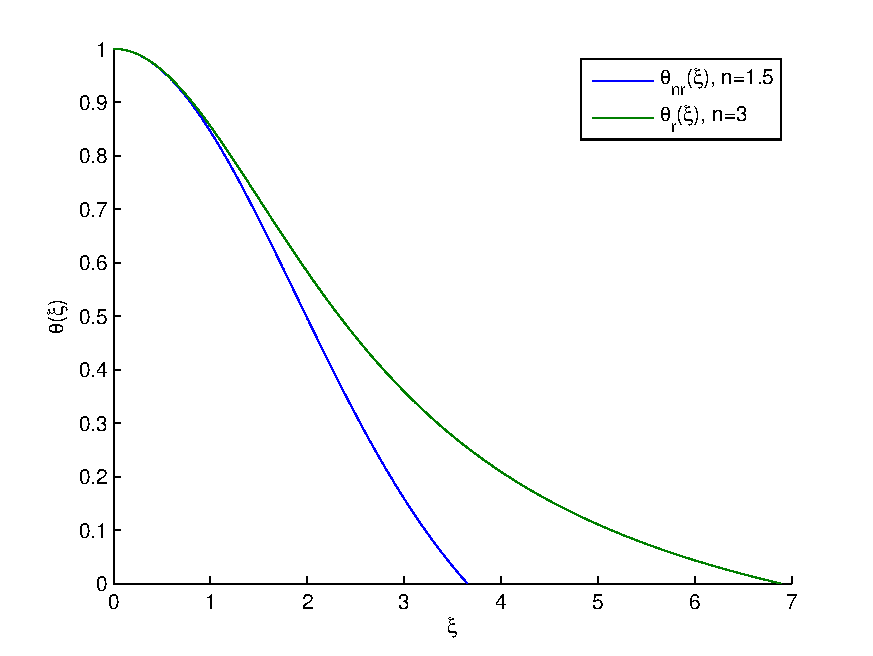
\includegraphics[width=0.55\textwidth]{lesolution.pdf}
\end{figure}

The first physically meaningful relationship that is most readily found from the
polytrope is the density profile of the star; the relationship between density
and radius. Obtaining this relationship in dimensionless form is just a matter
of using the definition of \(\theta\):

    \begin{equation}
        \theta^n=\frac{\rho}{\rho_c}
    \end{equation}

then plotting \(\theta^n\) vs. \(\xi\):

\begin{figure}[H]
    \caption{Density relation}
    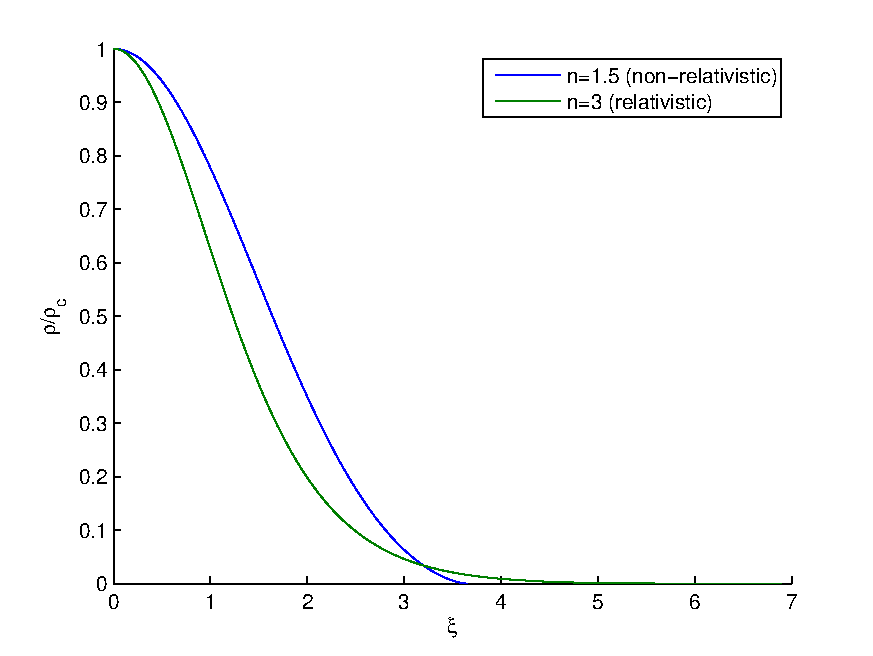
\includegraphics[width=0.55\textwidth]{density.pdf}
\end{figure}

Here we see that for a completely relativistic degenerate gas, the density
initially falls off more quickly with increasing radius than for a
non-relativistic gas, but this dropoff slows considerably near the stellar
surface resulting in a radius almost twice as large as the non-relativistic
case.


A plot of our initial attempt at a mass/radius relation compared with actual
data obtained from astronomical surveys\footnote{see Appendix B} shows the severe problems with the
model:

\begin{figure}[H]
    \caption{Incorrect mass/radius relation}
    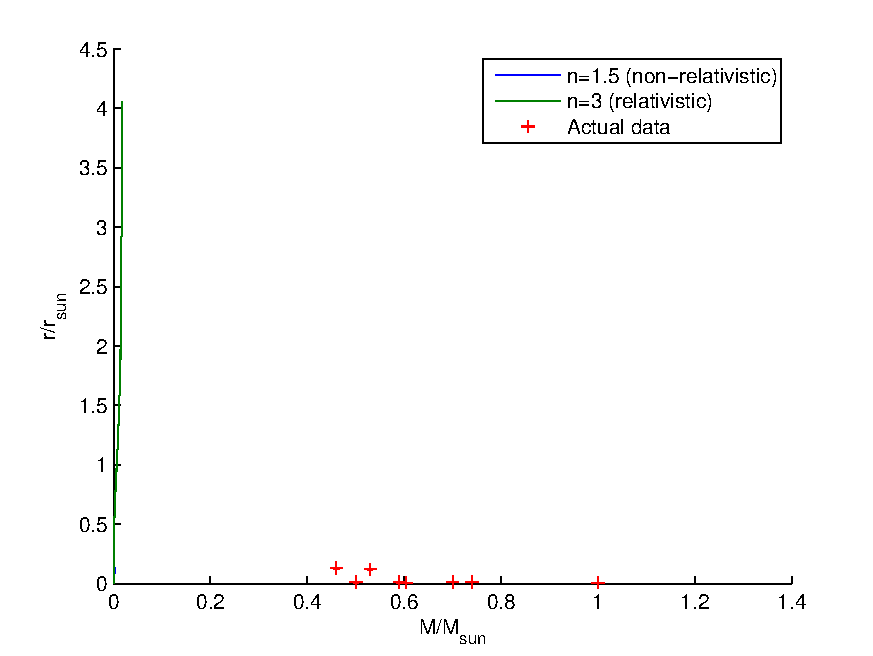
\includegraphics[width=0.55\textwidth]{mr-data.pdf}
\end{figure}

We do not see the expected constant value for the relativistic mass, and the
shapes of the relations do not match expectations (we should be seeing the
radius \emph{decrease} with increasing mass).

After fixing our procedure, we find the expected relation. The relativistic
polytrope results in a constant mass of \(1.4373 \textrm{M}_{\odot}\), which rounds to
the expected value of \(M_C=1.44 \textrm{M}_{\odot}\).

We then combined the relativistic and non-relativistic models by forcing the
radius to go to zero at the Chandrasekhar mass (values in this relation are from
the non-relativistic and relativistic mass/radius relations, with \(w\) as a
combination constant:

\[ R=\sqrt{w\left(\frac{1}{G^2M_C^4}\right) -
\frac{5.4707\e{12}}{M_C^(8/3)/4.7338\e{16}M_C^{10/3}}} \]

We used a bisection algorithm to find the value of \(w\) that results in a root
at \(M=M_C\).

Plotting the combined model against observed data, we find that it fits better
than the non-relativistic model at larger masses:

\begin{figure}[H]
    \caption{Mass/radius relation for non-relativistic \& combined pressures
    with data}
    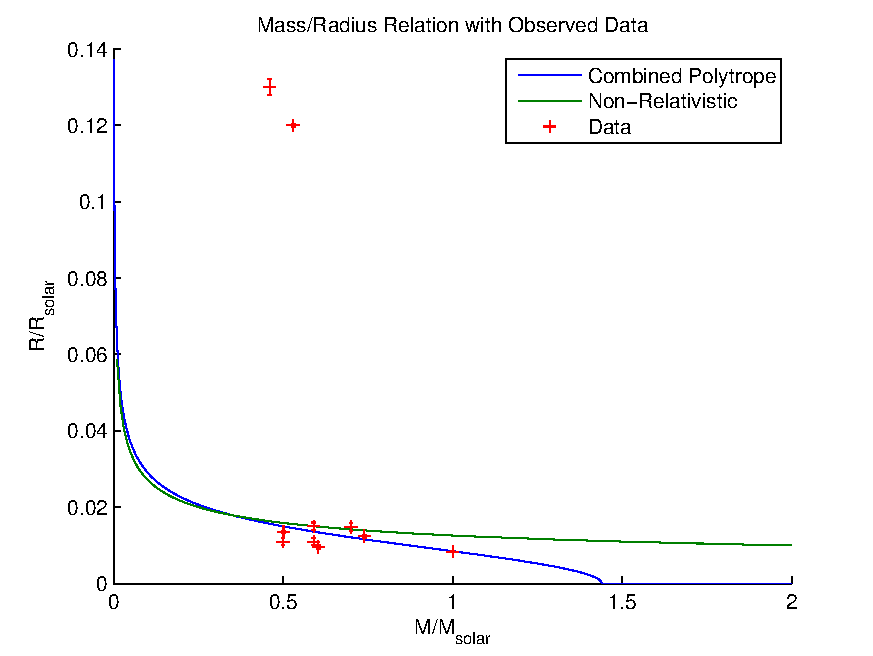
\includegraphics[width=0.55\textwidth]{mr_data_fixed.pdf}
\end{figure}

%------------------------------------------------

\section{Discussion}

\end{multicols}
%----------------------------------------------------------------------------------------
%	REFERENCE LIST
%----------------------------------------------------------------------------------------

\bibliographystyle{abbrv}
\bibliography{poly}
%----------------------------------------------------------------------------------------
%   APPENDICES
%----------------------------------------------------------------------------------------
\appendix
\appendixpage
\section{Derivation of the Lane-Emden Equation\cite[pp.176--179]{leblanc2010}} 

The Lane-Emden equation can be derived multiple ways; one way is from the
equations for hydrostatic equilibrium and mass conservation:

\begin{equation}
    \label{eq:hydroeq}
    \frac{dP(r)}{dr} = -\frac{\rho(r)GM(r)}{r^2}
    \end{equation}

    \begin{equation}
    \label{eq:masscons}
    dM(r)=4\pi r^2\rho(r)dr \rightarrow \frac{dM(r)}{dr} = 4\pi r^2\rho(r)
    \end{equation}

where \(P(r)\) is the gas pressure as a function of radial distance from the
center of the distribution, \(\rho(r)\) is the gas density, \(G\) is Newton's
gravitational constant, and \(M(r)\) is the mass enclosed within a sphere of
radius \(r\).

These equations can be related by multiplying eq.~\ref{eq:hydroeq} by
\(r^2/\rho\):

\[ \frac{r^2}{\rho(r)}\frac{dP(r)}{dr} = -\frac{r^2}{\rho(r)}
\frac{\rho(r)GM(R)}{r^2} \]

then differentiating with respect to \(r\):
            
\[
\frac{d}{dr}\left(\frac{r^2}{\rho(r)}\frac{dP(r)}{dr}\right)=-G\frac{dM(r)}{dr}
\]

Substituting in eq.~\ref{eq:masscons} we obtain Poisson's equation for gravitational potential:

\begin{equation}
    \label{eq:poisson}
    \frac{1}{r^2} \frac{d}{dr} \left( \frac{r^2}{\rho(r)}\frac{dP(r)}{dr} \right) = -4 \pi G\rho(r)
\end{equation}

Now, using the polytropic state equation:

\begin{equation}
    \label{eq:polytropstate}
    P=K\rho^{\frac{n+1}{n}}
\end{equation}

where \(n\) is called the \textit{polytropic index} and \(K\) is a constant, and
defining a dimensionless function \(\theta(r)\):

\begin{equation}
    \label{eq:thetar}
    \rho(r)=\rho_c\theta^n{r}
\end{equation}

where \(\rho_c\) is the central density of the star, we can rewrite the pressure
as a function of \(\theta(r)\):

            \[
                P(r)=K\rho_c^{\frac{n+1}{n}}\theta^{n+1}(r)=P_c\theta^{n+1}(r)
            \]

            where \(P_c=K\rho_c^{\frac{n+1}{n}}\) is the central pressure of the
            star. Substituting this into eq.~\ref{eq:poisson}:

            \[
                K\rho_c^{\frac{n+1}{n}}\frac{1}{r^2}\frac{d}{dr}\left(\frac{r^2}{\rho_c\theta^n(r)}\frac{d\theta^{n+1}(r)}{dr}\right)=-4\pi
                G\rho_c\theta^n(r)
            \]

            This can be simplified a bit by realizing that
            \(\frac{d\theta^{n+1}(r)}{dr}=(n+1)\theta^n(r)\frac{d\theta(r)}{dr}\):

            \begin{equation}
                \label{eq:simplpois}
                \frac{(n+1)P_c}{4\pi
                G\rho_c^2}\frac{1}{r^2}\frac{d}{dr}\left(r^2\frac{d\theta(r)}{dr}\right)=-\theta^n(r)
            \end{equation}

            Since we defined \(\theta(r)\) as a dimensionless function, this
            equation requires that \(\frac{(n+1)P_c}{4\pi G\rho_c^2}\) has the
            dimension of length squared. For further simplification, we can
            define a new constant factor \(\alpha\) that depends on the
            polytropic index \(n\):

            \begin{equation}
                \label{eq:alpha}
                \alpha^2=\frac{(n+1)P_c}{4\pi G\rho_c^2}
            \end{equation}

            and a new dimensionless radius \(\xi\):

            \begin{equation}
                \label{eq:xi}
                \xi=\frac{r}{\alpha}
            \end{equation}

            Substituting this \(\xi\) into eq.~\ref{eq:simplpois} we finally
            obtain the Lane-Emden equation:

            \begin{equation}
                \frac{1}{\xi^2}\frac{d}{d\xi}\left(\xi^2\frac{d\theta(\xi)}{d\xi}\right)=-\theta^n(\xi)
            \end{equation}

\section{Data Tables}

\begin{table}[H]
    \caption{Observed masses and radii for white dwarfs}
    \centering
    \begin{tabular}{c c c}
    \toprule
    %\multicolumn{2}{c}{Name} \\
    %\cmidrule(r){1-2}
    Name & Mass & Radius \\
         & \(\mathrm{M}_{\odot}\) & \(\mathrm{R}_{\odot}\) \\
    \midrule
    Sirius B & \(1.000\pm0.016\) & \(0.0084\pm0.0002\) \\
    Procyon B & \(0.604\pm0.018\) & \(0.0096\pm0.0004\) \\
    40 Eri B & \(0.501\pm0.011\) & \(0.0136\pm0.0002\) \\
    CD-38 10980 & \(0.74\pm0.04\) & \(0.01245\pm0.0004\) \\
    W485A & \(0.59\pm0.04\) & \(0.0015\pm0.001\) \\
    L268-92 & \(0.70\pm0.12\) & \(0.0149\pm0.001\) \\
    L481-60 & \(0.53\pm0.05\) & \(0.1200\pm0.0004\) \\
    G154-B5B & \(0.46\pm0.08\) & \(0.13\pm0.002\) \\
    G181-B5B & \(0.50\pm0.05\) & \(0.011\pm0.001\) \\
    G156-64 & \(0.59\pm0.06\) & \(0.011\pm0.001\) \\
    \bottomrule
    \end{tabular}
\end{table}


\end{document}
